\chapter{Auswertung}

Nach der Herstellung der bei einigen Proben ohne Zuhilfenahme von Hilfsmitteln das Vorhandensein der Gitterstruktur zu erkennen. Beim Betrachten der Proben unter bestimmten Winkeln war die Brechung des Lichtes durch das Gitter zu beobachten.

Eine Betrachtung der Proben unter dem Lichtmikroskop f�hrte zu keinen Ergebnissen. Die Aufl�sung des Lichtmikroskops ist zu gering um die hergestellten Gitterstrukturen aufl�sen zu k�nnen (vgl. Abbildung \ref{fig:nix}). Gitterstrukturen mit einer Periode von 400~nm sind gerade noch vom Lichtmikroskop aufzul�sen. Abbildung \ref{fig:400nm}\footnote[1]{Probe Hergestellt von Uwe Bog} zeigt ein solches Gitter unter 100-facher Vergr��erung.

\begin{figure}%
\centering
%\begin{adjustwidth}{0cm}{0cm}
	\subfloat[]{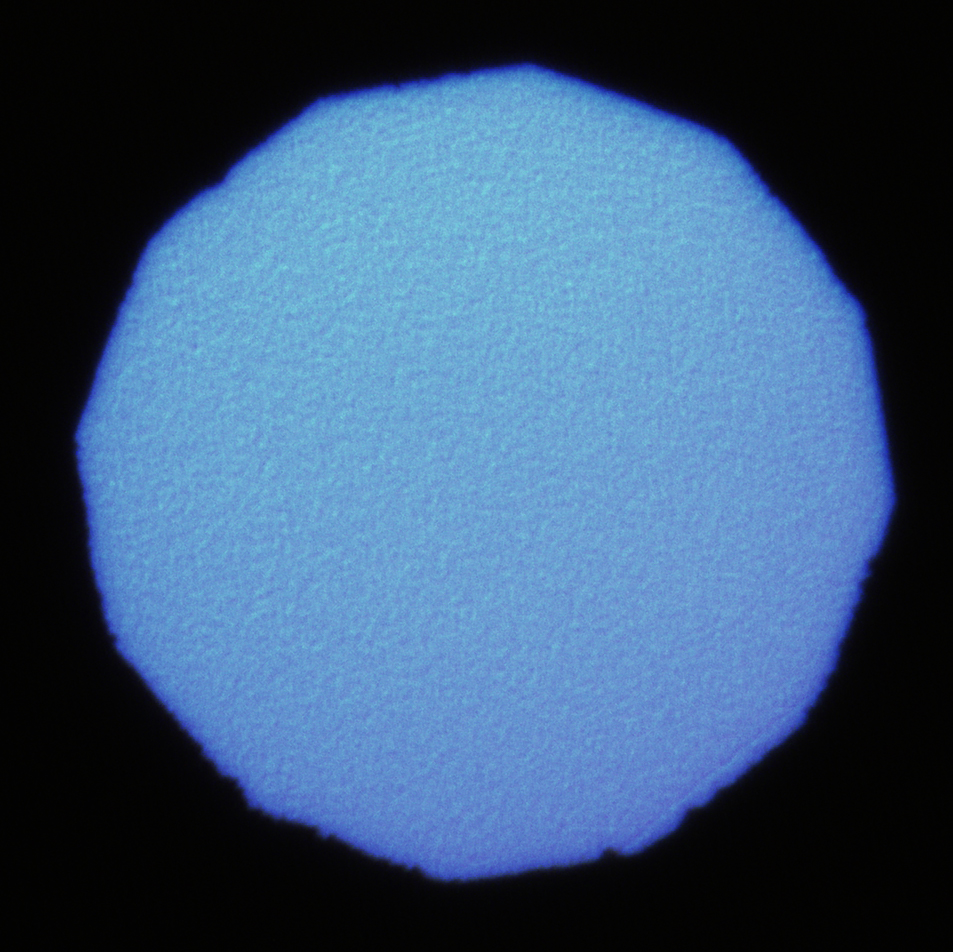
\includegraphics[totalheight=5 cm]{Grafiken/nix.jpg}\label{fig:nix}}\qquad
	\subfloat[]{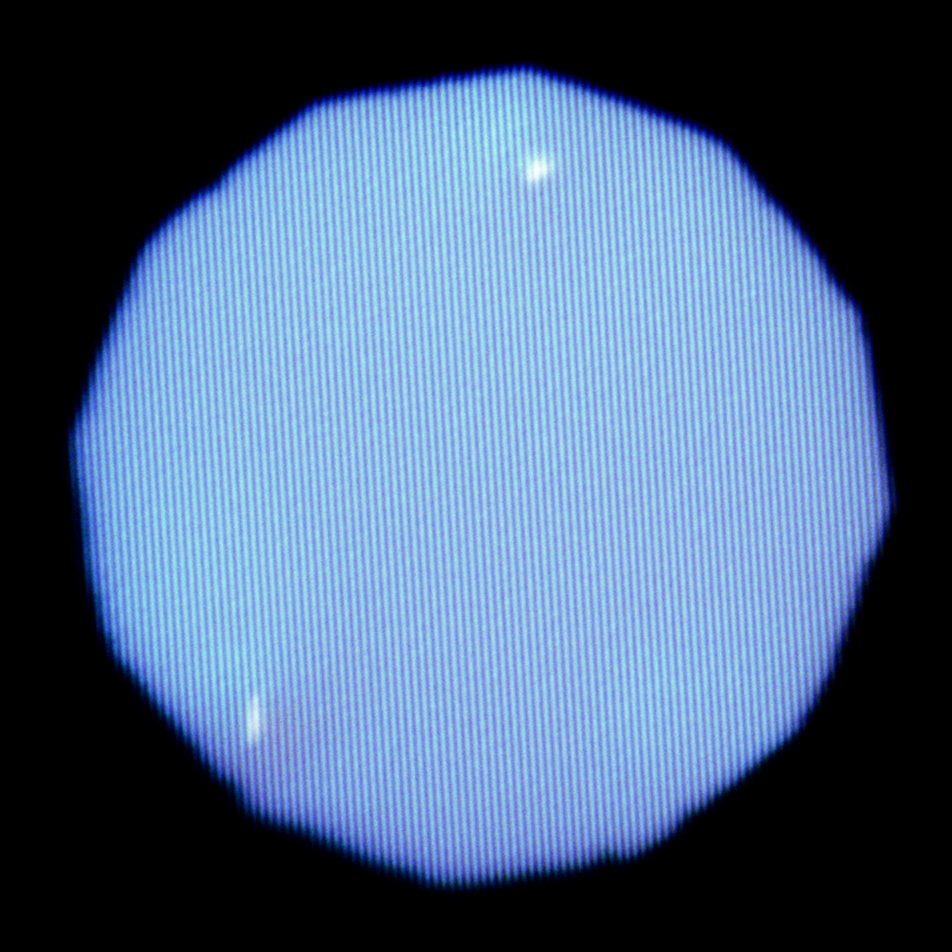
\includegraphics[totalheight=5 cm]{Grafiken/400nm.jpg} \label{fig:400nm}}\\%
%\end{adjustwidth}
\caption{Proben unter dem Lichtmikroskop. \textbf{(a)} Die Aufl�sung des Lichtmikroskops reicht nicht aus um die Strukturen aufzul�sen. \textbf{(b)} Gitterstruktur mit einer Periodizit�t von 400~nm.$^1$}%
\label{fig:matlab}%
\end{figure}



Um die hergestellten Proben zu Charakterisieren wurden die Proben am Institut f�r Mikrosystemtechnik (IMT) mit einem \textit{Atomic Force Microscope} (AFM) vermessen. Abbildung \ref{fig:3d_bild} zeigt die mit dem AFM Topografie einer hergestellten Gitterstruktur.

\begin{figure}%
\centering
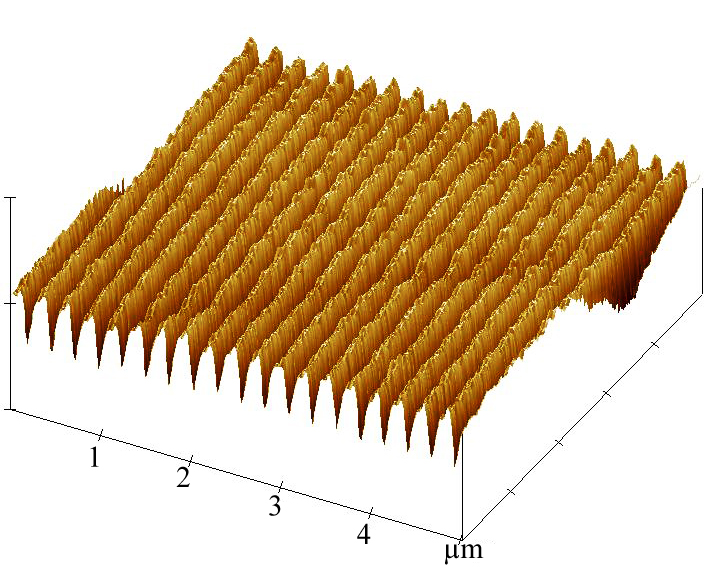
\includegraphics[width=.65\columnwidth]{Grafiken/3d_bild.jpg}%
\caption{AFM Messung der Topografie einer hergestellten Gitterstruktur (40~mJ, 4~s Entwicklungszeit).}%
\label{fig:3d_bild}%
\end{figure}

Die Gitterstrukturen wurden damit Vermessen. Jede Probe wurde an mehreren Positionen durch das AFM abgetastet. Abbildung \ref{fig:vgl_periode} zeigt Messungen zweier Proben. \ref{fig:periode1} 
\begin{figure}%
\centering
%\begin{adjustwidth}{0cm}{0cm}
	\subfloat[40~mJ, 5~s]{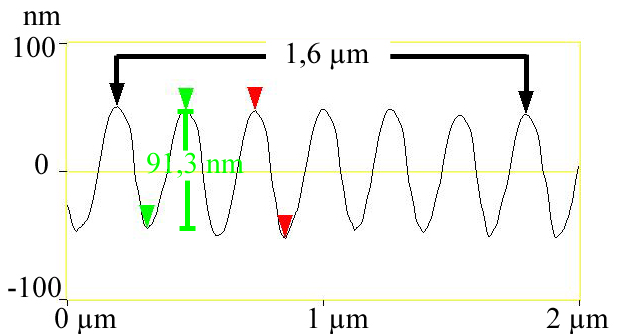
\includegraphics[totalheight=4 cm]{Grafiken/Periode_40mj_5s_1.jpg}\label{fig:periode1}}
	\subfloat[20~mJ, 10~s]{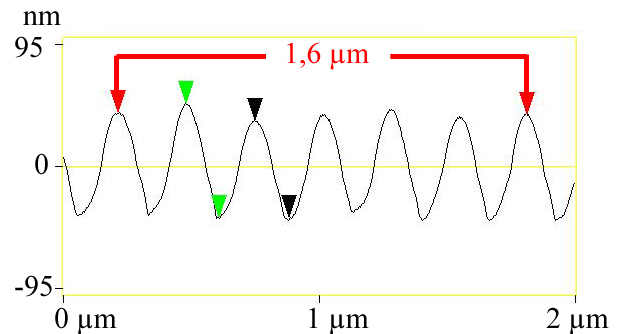
\includegraphics[totalheight=4 cm]{Grafiken/Periode_20mj_10s_w1.jpg} \label{fig:periode2}}
%\end{adjustwidth}
\caption{Mit dem AFM gemessene Gittertopographien. Gitterperiode beider Proben: $\sim$267~nm. \textbf{(a)} Dosis: 40~mJ, Entwicklungszeit: 5~s. \textbf{(b)} Dosis: 20~mJ, Entwicklungszeit 10~s. }%
\label{fig:vgl_periode}%
\end{figure}


Im Folgenden sollen die Auswirkungen der Belichtungsdosis und der Entwicklungszeit auf die hergestellten Gitterstrukturen untersucht werden. Hierzu werden neben den im Rahmen des Laborversuches hergestellten Proben (vgl. Tabelle \ref{tab:parameter}) auch weitere Proben verwendet. Diese wurden im Labor Nanotechnologie von Matthias Ba�ler, Simon Jau� und Martin Waldvogel unter Anleitung von Uwe Bog hergestellt und vermessen wurden.\footnote[2]{Ba�ler, Jau�, Waldvogel; Pr�sentation zum Laboversuch Laser Interverenz Lithographie; 15.08.2011} Tabelle \ref{tab:Referenz} zeigt die Herstellungsparameter dieser Proben.

\begin{table}%
\centering
\caption{Von Laborgruppe ''Ba�ler``$^2$ hergestellte Proben.}
\begin{tabular}{cc}

\toprule
Entwicklungsdauer	& Belichtungsenergien\\
in s	& in mJ\\
\midrule
10 & 10, 40, 80\\
20  & 10, 40, 80\\
30 & 10, 40, 80\\
\bottomrule 
\end{tabular}
\label{tab:Referenz}
\end{table}

